\section{Communication in Spontaneous Wireless Networks}
\label{s:comm_wless}

This section describes the basics of communication between wireless devices and presents the main implications for spontaneous wireless networks at layer 3. Physical limitations and derived properties are examined in section \ref{s:phy}. The implications of these properties in the networking model for spontaneous wireless networks, and in particular the suitability of the IP model, are detailed in section \ref{ss:ip}, is discussed in section \ref{ss:issues}. Finally, section \ref{ss:model} describes an IP-compatible networking model for multi hop communication in spontaneous wireless networks.

\subsection{Physical Aspects of Wireless Communication}
\label{s:phy}

The fact that two wireless devices in a wireless network are able to communicate to each other depends of several factors (see Figure \ref{f:wlessab}), and some of them are not related to any of the involved devices. The most significant factors include:

\begin{enumerate}[(i)]
\item The distance between two devices.
\item The physical properties of the transmitting and receiving antennas: number of transmission/reception antennas, transmission power and antenna directivities.
\item Network dynamics: in mobile networks, depending on the relative motion of wireless devices involved in communication, the Doppler frequency shift may have a non-negligible impact.
\end{enumerate}

The modulation and coding schemes used to transmit and receive packets have impact in other physical factors of the transmission, including:

%\item The physical properties of the transmitting and receiving antennas and of the transmission itself: modulation scheme, transmission power, antenna directivities.

\begin{enumerate}[(i)]
	\setcounter{enumi}{3}
\item The characteristics of the wireless medium: signal frequency band, noise power, effect of weather conditions or {\em interferences} from other devices transmitting in close frequency bands.
\item The physical topology of the {\em coverage} area: fading caused by obstacles, reflection and absorption causing multi-path interference and signal loss.
%The state of the electromagnetic spectrum in the environment: weather conditions or interferences from other transmitters. 
\end{enumerate}

\begin{figure}
\centering
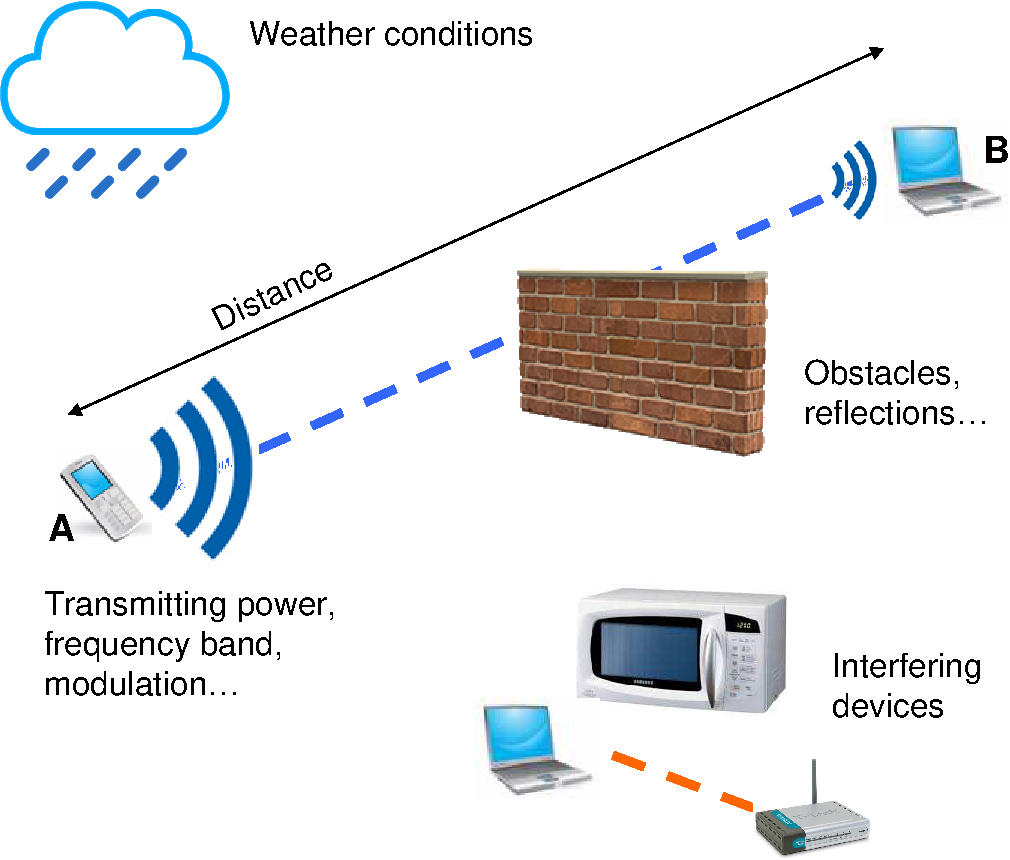
\includegraphics[width=0.60\textwidth]{Figures/wirelessab-crop.pdf}
\caption{Communication between wireless devices $A$ and $B$}
\label{f:wlessab}
\end{figure}

Note that, as some of these factors are time-variant and their impact may change rapidly, {\em e.g.} (iv), some links (or all of them) may have intermittent availability, even if devices keep static.

\paragraph{Coverage and Interference}

The concepts of {\em coverage} and {\em interference} have been mentioned in the previous list, and are some of the key parameters that define the behavior and impact of a wireless interface in a spontaneous wireless network.

\begin{definition}[Coverage Area]
Given a wireless interface $A$, the \emph{coverage area} of $A$ is the geographical region in which packets transmitted by $A$ can be received and correctly decoded by other interfaces on the same wireless medium as $A$, when no competing transmission is ongoing. The coverage area of $A$ is denoted by $Cov(A)$.
\end{definition}

\begin{definition}[Interference Area]
Given a wireless interface $A$, the \emph{interference area} of $A$ is the geographical region in which interfaces connected to the same wireless medium as $A$ may be unable to receive or correctly decode other packets when there is an ongoing transmission from $A$. The interference area of $A$ is denoted by $Intf(A)$.
\end{definition}

\begin{remark}
Note that, the coverage area of a wireless networking interface is always contained in the interference area of that interface, that is, $Cov(A) \subseteq Intf(A) \forall A$, as shown in the following and represented in Figure \ref{f:cov_intf}.
	\begin{itemize}
	\item Let $T>1$ be the SINR (Signal-and-Interferece-Noise-Ratio) threshold for receiving and decoding correctly packets from a wireless interface. That means that a transmission ({\em e.g.}, from $A$) is received and correctly decoded by the receiver, in absence of competing transmissions, if $\textrm{SINR}|_{I=0}=\textrm{SNR}=\frac{S}{N} > T$ and discarded otherwise. As received power decreases quadratically with distance from the transmitter, let $S(d)=\frac{P}{d^2}$. Then, the maximum coverage distance is $d_c=\sqrt{\frac{P}{NT}}$. The maximum distance at which there may be interference (from $A$), $d_i$, corresponds to the distance to a receiver $B$ such that another transmitter, $C$, transmitting with the same power $P$ at any distance $d\leq d_c$ from $B$, would be unable to send successfully a packet in case of concurrent transmission from $A$. This is, $T=\textrm{SINR}|_{N \ll I}=\textrm{SIR}=\frac{P/d_{BC}^2}{P/d_i^2}$. In the worst case, $d_{BC} = d_c$ and $\frac{P/d_{BC}^2}{P/d_i^2} = \frac{d_{i}^2}{d_c^2} = T$, and therefore $d_i<d_c$.
	\end{itemize}
\end{remark}

% added -------------------------------
\begin{comment}

\emph{Proposition \ref{p:cov_intf}} defines the coverage and interference areas under the conditions of the Friis' Transmission Equation (\ref{e:free}), and shows in particular that the latter is bigger than the former.

{\small
	\begin{theorem}
	\label{p:cov_intf}
	Let $a$ be a wireless interface in a wireless network, in which information propagates under free space conditions. Let $P$ be the power at which all interfaces transmit in the network, and $N$ the noise power, assuming an AWGN\footnote{Additive White Gaussian Noise.} model. Let $T>1$ be the minimum signal-to-interference-and-noise ratio (SINR) for a transmission to be successfully decoded by $a$. 
	Then, the coverage area of $a$ is a circle centered in $a$ with radius $r=4\pi \sqrt{\frac{P}{NT}}$, and the interference area of $a$ is a circle centered in $a$ with radius $r_i=4\pi\sqrt{\frac{P}{N}}$. As $T>1$, $r_i>r$.
	\end{theorem}
	\begin{proof} The coverage area of $a$ is the geographical region in which the SINR of the received signal is higher than $T$, in absence of other transmissions (def.~ \ref{d:cov}). If not other transmissions occur, there is no interference ($I=0$), and the SINR for an interface $b$, at distance $d$ of $a$ becomes the signal-to-noise ratio, SNR of $b$.
		\begin{equation*}
		SINR|_b = \left.\frac{S}{N+I}\right]_b = [I=0] = \left.\frac{S}{N}\right]_b = SNR|_b
		\end{equation*}
	Applying the Friis Transmission Equation (\ref{e:free}) and assuming unitary gains $G_r,G_t=1$,
		\begin{eqnarray*}
		SNR|_b = \left.\frac{S}{N}\right]_b > T \\
		\frac{P\left(\frac{\lambda}{4\pi d}\right)^2}{N} > T \\
		d < 4\pi \sqrt{\frac{P}{NT}} = r
		\end{eqnarray*}
	When $d<r$, an interface at distance $d$ from $a$ is able to receive packets transmitted from $a$.
	For the interference area (def.~ \ref{d:intf}), consider the case when an interface $b$ at distance $d$ receives signals from $a$ and from another (neighboring) interface, $c$, at distance $d_o$ from $b$. Transmission from $a$ causes interference with a transmission from $c$, in $b$, if the SINR at $b$ is lower than $T$. Considering that the impact of the noise is negligible with respect to interference ($N \ll I$):
		\begin{eqnarray*}
		SINR_b \approx SIR_b = \left.\frac{S}{I}\right]_b > T \\
		\frac{P\left(\frac{\lambda}{4\pi d}\right)^2}{P\left(\frac{\lambda}{4\pi d_o}\right)^2} > T \\
		d < d_o\sqrt{T}
		\end{eqnarray*}
	Consider the worst case: distance between $b$ and the main transmitter $c$ is maximum, \emph{i.e.}, $r=4\pi \sqrt{\frac{P}{NT}}$. Then:
		\begin{equation*}
		d < \frac{\lambda}{4\pi}\sqrt{\frac{P}{N}} = r_i
		\end{equation*}
	where $r_i$ is the radius of the interference area of $a$.
	\end{proof}
}

\end{comment}
% end added ---------------------------------------------

\begin{figure}[htb]	% H-must be here or [htb]
\centering
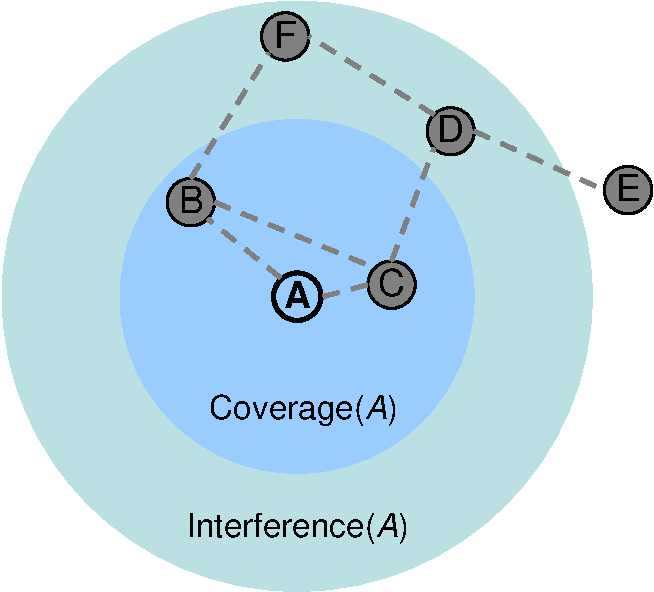
\includegraphics[width=0.40\textwidth]{Figures/cov_intf-crop.pdf}
\caption{Idealized representation of coverage and interference areas of an interface $A$.}
\label{f:cov_intf}
\end{figure}

Due to the variability of factors having impact on wireless communication, coverage and interference areas of an interface are time-variant and in practice their shapes are significantly more irregular than the circles depicted in Figure \ref{f:cov_intf} \cite{kotz03}. Even within the coverage area at a particular time, when communication is possible, a wireless link is inherently unreliable and prone to transmission errors and packet losses \cite{book_wless}, for instance due to interferences from other interfaces in the network or external sources transmitting in the same frequency band. 

\subsection{IP Model Issues in Spontaneous Wireless Networks}
\label{ss:issues}

The properties of wireless medium have severe implications for the characteristics of neighbor relationship at layer 3 (L3) in spontaneous wireless networks. In contrast to the case of wired IP links, neighbor relationships between wireless interfaces are not necessarily {\em symmetric} nor {\em transitive} \cite{baccelli12}. This entails some additional effect that are further illustrated in this section: the {\em hidden node} problem and the {\em exposed node} problem.

\begin{figure}[htb]	% H-must be here or [htb]
\centering
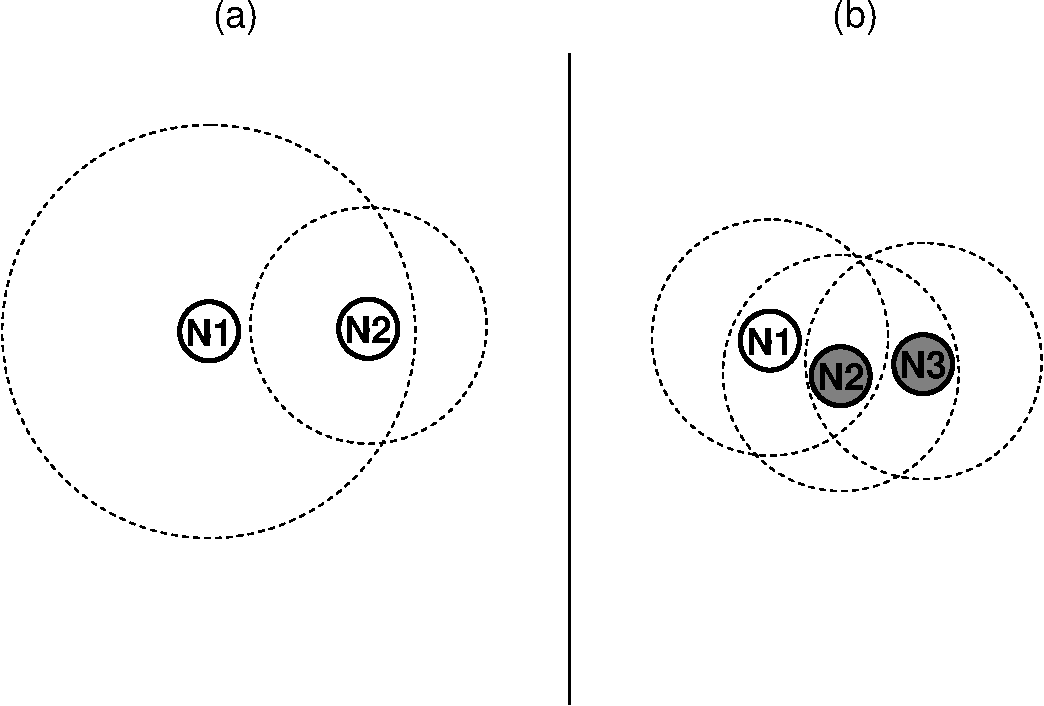
\includegraphics[width=0.7\textwidth]{Figures/asym-crop.pdf} \\
\caption{Asymmetry and non-transitivity in neighbor relationships between wireless interfaces.}
\label{f:asym}
\end{figure}

\paragraph{Non-Symmetric Links}

Consider the small wireless network in Figure \ref{f:asym}.a: for some reason (powerful transmitter, large antenna, ...) the wireless interface of $N1$ has a large enough coverage area that its transmissions can be received by the wireless interface $N2$. The wireless interface of $N2$, on the other hand, has a much smaller coverage radius, such that transmissions from the wireless interface of $N2$ do not arrive at the wireless interface of $N1$. Thus an asymmetric --or more precisely, an unidirectional-- connectivity between the wireless interface of $N1$ and the wireless interface of $N2$ exists: $N2$ sees $N1$ as a neighbor (since the wireless interface $N2$ can receive transmissions from the wireless interface of $N1$), whereas $N1$ does not see $N2$ as a neighbor (since the wireless interface of $N1$ can not receive transmissions from the wireless interface of $N2$). This situation illustrates that neighbor relationships in a wireless network are not necessarily symmetric.

\paragraph{Non-Transitive Links} Figure \ref{f:asym}.b shows a case of non-transitive links in a 2-hop wireless network. $N1$ and $N2$ are neighbors: the wireless interface of $N1$ is inside the coverage area of $N2$, and therefore $N1$'s transmissions are received at the wireless interface of $N2$ -- and viceversa. Observe that the same applies with $N2$ and $N3$: $N2$ and $N3$ are also neighbors. However, direct communication between $N1$ and $N3$ is not possible, as their respective wireless interfaces are outside the coverage area of each other. In a spontaneous wireless network, the fact that $N1$ and $N2$ are neighbors ({\em i.e.}, can communicate directly) and $N2$ and $N3$ are neighbors as well does not imply that $N1$ and $N3$ are neighbors to each other: neighbor relationship in a spontaneous wireless network is not necessarily transitive. \ \\ \ \\
%
These two constraints lead to situations that do not occur in traditional IP networks, such as the {\em hidden node problem} and the {\em exposed node problem}.

\begin{figure}[htb]	% H-must be here or [htb]
\centering
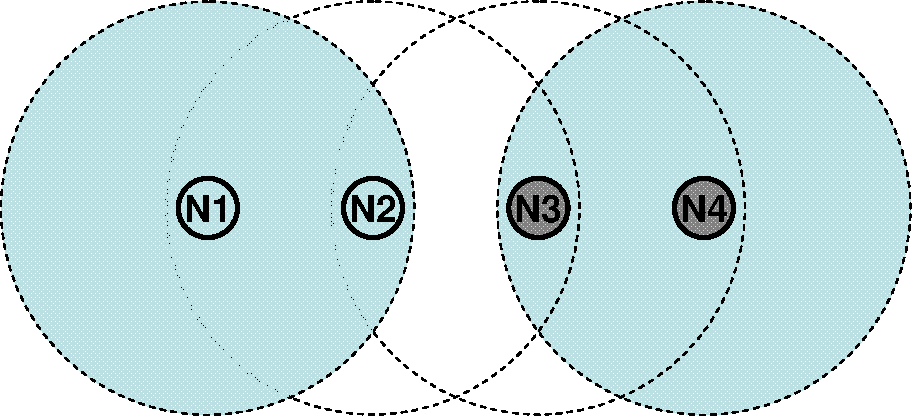
\includegraphics[width=0.6\textwidth]{Figures/four-crop.pdf} \\
\caption{A four-node wireless network, with the (idealized) coverage areas of its nodes.}
\label{f:4nodes}
\end{figure}

\paragraph{Hidden Nodes}

Consider the spontaneous wireless network represented in Figure \ref{f:4nodes}. If $N3$ agrees with its neighbours (N2 and $N4$) that it will, for the moment, have exclusive access to the wireless media via its wireless interface, then $N3$ may go ahead and make a transmission. However, if at the same time $N1$ also transmits over its wireless interface, then the transmissions of the wireless interfaces of $N1$ and $N3$ may appear concurrently at the wireless interface of $N2$ -- potentially interfering and causing $N2$ to receive neither of the transmissions. Denoted a {\em collision}, the possibility and probability of this occurring depends on the L2 (data link layer) mechanisms in place -- suffice to observe that such collisions can and do occur when using some common wireless interfaces such as IEEE 802.11. The term {\em hidden node} originates from the fact that while the node wishing exclusive access to the wireless media may negotiate this with its direct neighbours (in our case $N2$ and $N4$), nodes out of direct radio range (in our case $N1$) are {\em hidden} to the node requesting media access and cannot thus participate in the negotiation.

% (text from Thomas, from "A MANET Architecture Model", sec. 3.3)

\paragraph{Exposed Nodes}

This can be considered as the dual problem of the {\em hidden node} situation described above: an {\em exposed node} is a node that is prevented to transmit due to the transmission of a neighbor, even when the two transmissions would not be interfer. Consider again the network of Figure \ref{f:4nodes}. In the moment in which $N3$ starts a transmission, after having agreed the exclusive use of the wireless channel with neighbors $N2$ and $N4$, $N2$ is an {\em exposed node} because it is not able to transmit during the transmission of $N3$, in order to avoid collisions. Note however that not all concurrent transmissions from $N2$ would cause collision with the ongoing transmission from $N2$ to $N4$ -- in particular, there are no collisions if destinations do not receive several packets at the same time: a packet transmission from $N3$ to $N4$ and from $N2$ to $N1$ would not cause any collision. The {\em exposition} of $N2$ to the transmission of $N3$ entails thus a reduction in the available bandwidth. \ \\ \ \\
%
% (text from Thomas, from "A MANET Architecture Model", sec. 3.4)
%
The hidden and exposed node problems are consequences of the fact that links between wireless interfaces in a spontaneous wireless network are not necessarily symmetric or transitive. These are major differences with the IP networking model (see section \ref{ss:ip}), in which neighbor relationships inside an IP link are assumed to be symmetric and transitive. As these assumptions do not hold necessarily in spontaneous wireless networks, {\em wireless links in a spontaneous wireless network should not be directly modeled, in general, as IP links} \cite{softcom09}.

%{\bf Implications in addressing.-}

\subsection{An IP-compatible Architectural Model}
%\subsection{A Model for Nodes and Interfaces in Wireless Multi-Hop Ad hoc Networks}
\label{ss:model}

%This section presents the main elements of a networking model for spontaneous wireless networks and nodes \cite{tc_manetarch} that enables the compatibility of IP with the characteristics of spontaneous wireless networks. 

This section derives from the previously-described observations a general IP-compatible networking model for spontaneous wireless networks \cite{tc_manetarch}. This model enables the compatibility of IP with the characteristics of spontaneous wireless networks, without relying on assumption concerning topology or capabilities of wireless links.

\paragraph{Network View}

IP operating on a spontaneous wireless network can be conceived in two separate levels, as represented in Figure \ref{f:manetview}: the level of traditional IP networking, and the level in which wireless interfaces are connected in a spontaneous wireless network. 
\begin{itemize}
\item The first level (inner white cloud in Figure \ref{f:manetview}) contains {\em wireless interfaces} from routers that communicate with each other by way of {\em wireless links}, and form a spontaneous wireless network with the non-standard properties described throughout this section. Wireless interfaces in this level present {\em semibroadcast} communication properties (see paragraph below) and are therefore not required to satisfy the conditions of IP links. 
\item The second level (outer gray cloud in Figure \ref{f:manetview}) contains the links between routers and hosts, in which the classic IP link model, as described in section \ref{ss:ip}, applies.
\end{itemize}

%Following the architecture described in this section, a configured wireless multi-hop network with routers and hosts is splitted in two separate levels: the level of traditional IP networking, and the level in which wireless interfaces are connected in a wireless multi-hop ad hoc network. Figure \ref{f:manetview} represents this two-level structure: the inner white cloud represents the level where semibroadcast interfaces and links form a wireless multi-hop ad hoc network -- and the outer gray cloud represents the level where the classic IP link model, as described in section \ref{ss:ip}, applies.

\begin{figure}[htb]	% H-must be here or [htb]
\centering
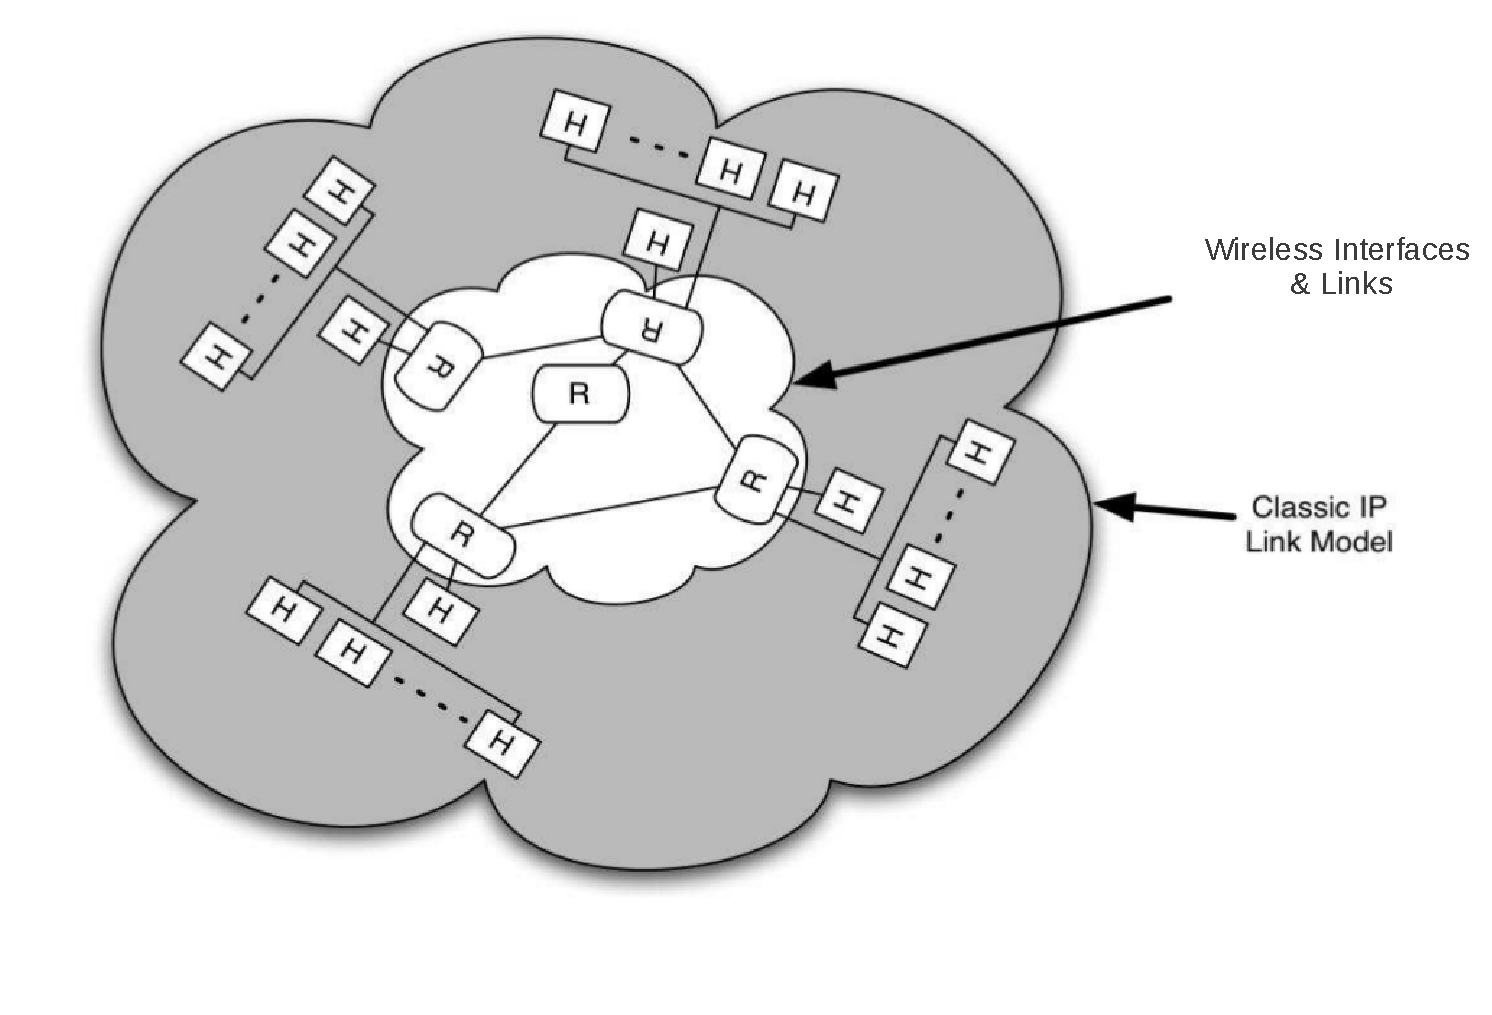
\includegraphics[width=0.75\textwidth]{Figures/manetview3-crop.pdf} \\
\caption{A view of a spontaneous wireless network, following the architecture model described in this section.}
\label{f:manetview}
\end{figure}

% (text from Thomas, from "A MANET Architecture Model", sec. 5.4)

\paragraph{Semibroadcast Interfaces}

As mentioned in section \ref{s:phy}, packets transmitted by a wireless interface $A$ are simultaneously received by the set of wireless interfaces within the coverage area of $A$, and can be successfully decoded by all those receiving interfaces for which no other transmission causes interference. In a spontaneous wireless network, this set does not contain in general all interfaces in the network. Moreover, as links are not necessarily symmetric in wireless networks and interface coverage areas have a time-variant, irregular arbitrary shape \cite{kotz03}, packets from an interface that has received and correctly decoded packets from $A$ are not guaranteed to be received and correctly decoded by $A$. Wireless {\bf semibroadcast interfaces} are thus ``broadcast-capable interfaces that {\em may} exhibit asymmetric reachability" (as defined in {\tt draft-ietf-autoconf-manetarch} \cite{ietf_manetarch}) and {\em may} not reach all interfaces in the spontaneous wireless network.

%Wireless interfaces in a wireless multi-hop ad hoc network can communicate with other interfaces (neighbors) within their coverage area. Although typically represented as a fixed radius circle around the interface (as in Figures \ref{f:cov_intf}, \ref{f:asym} and \ref{f:4nodes}), the coverage area of an interface has a time-variant, irregular arbitrary shape \cite{kotz03} -- so neighbor sets, even in a static network, are dynamic. These characteristics make possible for an interface to reach several neighboring interfaces in a single wireless transmission -- these interfaces are denominated {\bf semibroadcast interfaces} \cite{ietf_manetarch}.

%As the coverage area of different interfaces is not necessarily the same, wireless links are {\em not necessarily symmetric}: if an interface $A$ is within the coverage area of $B$, but $B$ is not included in the coverage area of $A$, then there is a link $B\longrightarrow A$, but the symmetric link $A \longrightarrow B$ does not exist. The neighborhood relationships are {\em not necessarily transitive}: the fact that an interface $A$ can communicate directly with another interface $B$, and that $B$ can communicate directly with $C$, does not imply that $A$ and $C$ can communicate directly. 

\paragraph{Node Morphology}

It has been mentioned (see section \ref{ss:spontaneous}) that nodes in a spontaneous wireless network can behave simultaneously as routers and hosts, in contrast to traditional wired computer networks which enforce a clear separation between host and router roles. A first intuition deriving from this observation leads to consider nodes in a spontaneous wireless network as standard hosts with routing capabilities, with an IP subnet prefix assigned to their wireless (semibroadcast) interfaces. This intuition however assumes implicitly that the semibroadcast interface of the router is attached to the IP link over which the host is configured (and receives its prefix), which is not consistent with the differences between IP links and links between interfaces in spontaneous wireless networks, detailed in section \ref{ss:issues}. %\ \\ \ \\
%
Instead, an alternative node model is proposed, which is compatible with the specific characteristics of links between semibroadcast interfaces, and consistent with the two-level network view described above in this subsection. In this model, a node virtually contains {\em one} router with a wireless interface to interact with the rest of wireless interfaces. As shown throughout this section, links between these wireless interfaces have semibroadcast properties and hence, cannot be configured, in general, as standard IP links in a straightforward manner. A node may also contain one or more hosts: if it does, its hosts belong to the {\em second level} of the network architecture (see Figure \ref{f:manetview}). This entails that the links between these hosts and the corresponding router are standard IP links. Figure \ref{f:node} illustrates the case of a node formed by a router $R$ with a wireless (semibroadcast) interface, and three hosts $H_1$, $H_2$ and $H_3$ connected to $R$ via standard IP links.

%As an IP link cannot be successfully built on top of a wireless multi-hop ad hoc network, as shown in section \ref{ss:issues}, this section proposes the inverse approach, that is, to build a wireless multi-hop network that connects wireless (semibroadcast) interfaces belonging to {\em nodes} that contain IP networks as described in Figure \ref{f:node}.

\begin{figure}[htb]	% H-must be here or [htb]
\centering
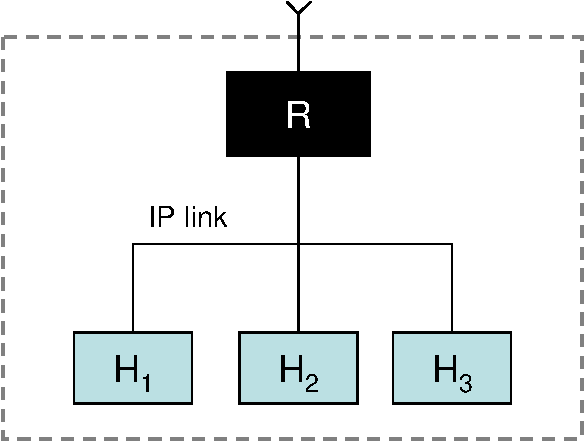
\includegraphics[width=0.35\textwidth]{Figures/manet_node-crop.pdf} \\
\caption{A node model for a spontaneous wireless network.}
\label{f:node}
\end{figure}

This implies that, from the point of view of the hosts, and the applications running on these hosts, connectivity is via a classic IP link. Host applications can thus run unaltered over spontaneous wireless networks, as the specificities of wireless semibroadcast communication have no architectural implications over the links through which hosts are connected: they remain architecturally banished to the {\em first level} depicted in Figure \ref{f:manetview}, and handled by wireless interfaces of the routers to which hosts are connected. Characteristics of multi-hop wireless communications can however still impact end-to-end performance experienced by hosts -- for instance, TCP may not be able to function as expected \cite{gerla99}. \ \\ \ \\
%
With this model, nodes in spontaneous wireless networks can behave simultaneously as hosts (that is, being source or destination of traffic) and as routers (forwarding other's traffic towards its destination), but hosts and routers interface differently with the rest of the network: hosts are connected to a classic IP link, while routers are connected to the spontaneous network by way of a semibroadcast interface over links that cannot be assumed symmetric or transitive, for instance.

%--- characteristics of wireless multi-hop ad hoc networks has no architectural effect in 

%are not exposed to the specific characteristics of the wireless semibroadcast interfaces and are connected to the wireless multi-hop network via a router, which has one or more wireless interfaces.

%This implies that, from the point of view of the hosts, and the applications running on these hosts, connectivity is via a classic IP link. Hosts, and their applications, are not exposed to the specific characteristics of the wireless semibroadcast interfaces and are connected to the wireless multi-hop network via a router, which has one or more wireless interfaces.

% (text from Thomas, from "A MANET Architecture Model", sec. 5.1)

\paragraph{Impact on IP Addressing}

IP addressing model is tied to the notion of IP link, as shown in section \ref{ss:ip}. As the assumptions underlying IP links do not hold in general on links between wireless interfaces, IP links should not be configured by default in spontaneous wireless networks \cite{rfc5889}. There are two major implications on not configuring IP links on such a network:

\begin{itemize}
\item {\bf Unique Prefixes}. Wireless interfaces must be configured with unique prefixes, {\em i.e.} such that no two wireless interfaces are configured such that they appear within the same IP subnet. Some common ways to achieve this are:

\begin{itemize}
\item unnumbered interfaces (IPv4) \cite{rfc1812};
\item Link-Local Addresses (IPv6);
\item full length prefixes: /128 (IPv6) or /32 (IPv4) prefixes.
\end{itemize}

However it is worth noting that prefix lengths shorter than /128 (IPv6) or /32 (IPv4) are possible on the semibroadcast interface, as long as the prefixes are unique to a single wireless interface.

\item {\bf Link Local Multicast/Broadcast Scope}. On a wireless interface, a Link Local multicast or broadcast reaches wireless interfaces of neighbor nodes only, regardless of their configured addresses. A Link Local multicast or broadcast on a wireless interface is, thus, a "neighborcast", and is not forwarded nor assumed to be received by all nodes within a spontaneous wireless network. \\
\end{itemize}  

% (text mostly from Thomas, from "A MANET Architecture Model", sec. 5.3)

The principles of the model described in this section have a concrete impact on spontaneous wireless networks operation as described in the remainder of the chapter. On one hand it specifies how IP interfaces should be configured on such networks, and on the other hand it identifies the need for novel protocols and the exact scope of their operation -- the {\em first level} depicted in Figure \ref{f:manetview}. The following sections will describe techniques and protocols for enabling communication at layer 3 in spontaneous wireless networks, within the scope of the {\em first level} shown in Figure \ref{f:manetview}. When needed, assumptions beyond those described in this model will be explicitly detailed in the corresponding protocols.
